\newpage
IRSTI 55.39.01

\sectionwithauthors{N.T. Smailova, A.Y. Popov}{bfseries ENSURING RELIABLE AND SAFE OIL STORAGE IN THE REPUBLIC OF KAZAKHSTAN}

\begin{center}
{\bfseries \textsuperscript{1}N.T. Smailova\textsuperscript{🖂}, A.Y.
Popov\textsuperscript{2}}

\textsuperscript{1} Kazakh University of Technology and Business named
after K.Kulazhanov, Astana, Kazakhstan

\textsuperscript{2} Omsk State Technical University, Omsk, Russian
Federation

{\bfseries \textsuperscript{🖂}}Correspondent-author: ganibek2006@mail.ru
\end{center}

The article highlights the issue of possible construction of the first
large oil storage facility in the history of Kazakhstan. Construction of
large oil storage facilities in Kazakhstan is an important step to
ensure efficient storage and management of oil products in the country,
solving the problem of redistribution and storage of oil products, given
the dynamics of production and consumption growth in the country.
Construction of a large oil storage facility in Atyrau region, as well
as oil depots in the west of Kazakhstan, will optimize the processes of
transportation and storage of oil products, reduce the cost of renting
other people\textquotesingle s storage facilities and ensure the
sustainability and reliability of oil products supplies to both domestic
and foreign markets. The article considers such important aspects as the
need for storage of oil products, technical and environmental aspects of
construction, as well as economic and social feasibility. In addition,
the article presents a system analysis and study of the potential for
construction of a large oil storage facility in Kazakhstan, which makes
it significant and relevant in the context of the development of the
country\textquotesingle s oil and gas industry. Given the current global
challenges, such as oil production limitations and volatility of oil and
oil products markets, the strategic reserve becomes even more relevant.

{\bfseries Key words:} hydrocarbon feedstock, storage of petroleum
products, strategic reserve, provision of domestic needs.

\sectionheading{ҚАЗАҚСТАН РЕСПУБЛИКАСЫНДА МҰНАЙДЫҢ СЕНІМДІ ЖӘНЕ ҚАУІПСІЗ САҚТАЛУЫН ҚАМТАМАСЫЗ ЕТУ}

\begin{center}
{\bfseries \textsuperscript{1}Н.Т. Смайлова\textsuperscript{🖂},
\textsuperscript{2}А.Ю. Попов}

\textsuperscript{1} Қ. Құлажанов атыңдағы Қазақ технология және бизнес
университеті, Астана, Қазақстан,

\textsuperscript{2}Омбы мемлекеттік техникалық университеті, Омбы,
Ресей,

email: ganibek2006@mail.ru
\end{center}

Мақалада Қазақстан тарихындағы алғашқы ірі мұнай қоймасын салу
мүмкіндігі туралы мәселе көтерілген. Қазақстанда ірі мұнай қоймаларының
құрылысы республикада мұнай өнімдерін тиімді сақтау мен басқаруды
қамтамасыз ету, мұнай өнімдерін қайта бөлу және сақтау мәселесін шешу,
мұнай өнімдерін өндіру мен тұтынудың өсу динамикасын ескере отырып,
маңызды қадам болып табылады. Атырау облысында ірі мұнай сақтау
қоймасының, сондай-ақ Қазақстанның батысындағы мұнай базаларының
құрылысы мұнай өнімдерін тасымалдау және сақтау процестерін
оңтайландыруға, шетелдік қоймаларды жалға алу құнын төмендетуге және
жеткізілімдердің тұрақтылығы мен сенімділігін қамтамасыз етуге мүмкіндік
береді және мұнай өнімдерін ішкі және сыртқы нарыққа шығару. Мақалада
мұнай өнімдерін сақтау қажеттілігі, құрылыстың техникалық және
экологиялық аспектілері, сондай-ақ экономикалық және әлеуметтік
орындылығы сияқты маңызды аспектілер қарастырылады. Сонымен қатар,
мақалада Қазақстандағы ірі мұнай қоймасын салу әлеуетін жүйелі талдау
және зерделеу ұсынылған, бұл оны еліміздің мұнай-газ саласын дамыту
контекстінде маңызды және өзекті етеді. Мұнай өндіруді шектеу және мұнай
мен мұнай өнімдері нарығындағы құбылмалылық сияқты ағымдағы жаһандық
сын-қатерлерді ескере отырып, стратегиялық резерв бұрынғыдан да өзекті
бола түседі.

{\bfseries Түйін сөздер:} көмірсутегі шикізаты, мұнай өнімдерін сақтау,
стратегиялық резерв, ішкі қажеттіліктерді қамтамасыз ету.

\sectionheading{ОБЕСПЕЧЕНИЕ НАДЕЖНОГО И БЕЗОПАСНОГО ХРАНЕНИЯ НЕФТИ В РЕСПУБЛИКЕ КАЗАХСТАН}

\begin{center}
{\bfseries \textsuperscript{1}Н.Т.Смайлова\textsuperscript{🖂},
\textsuperscript{2}А.Ю.Попов}

\textsuperscript{1}Казахский университет технологии и бизнеса им. К.
Кулажанова,

г. Астана, Казахстан,

\textsuperscript{2}Омский государственный технический университет,
г.Омск, Россия,

email: ganibek2006@mail.ru .
\end{center}

В статье освещается вопрос возможного строительства первого в истории
Казахстана крупного нефтехранилища. Строительство крупных нефтехранилищ
в Казахстане представляет собой важный шаг для обеспечения эффективного
хранения и управления нефтепродуктами в стране, решение проблемы
перераспределения и хранения нефтепродуктов, учитывая динамику роста
производства и потребления в стране. Строительство крупного
нефтехранилища в Атырауской области, а также нефтебаз на западе
Казахстана, позволит оптимизировать процессы транспортировки и хранения
нефтепродуктов, снизить затраты на аренду чужих хранилищ и обеспечить
устойчивость и надежность поставок нефтепродуктов как на внутренний, так
и на внешний рынки. В статье рассматриваются такие важные аспекты, как
потребность в хранении нефтепродуктов, технические и экологические
аспекты строительства, а также экономическая и социальная
целесообразность. Кроме того, в статье представлен системный анализ и
исследование потенциала строительства крупного нефтехранилища в
Казахстане, что делает ее значимой и актуальной в контексте развития
нефтегазовой отрасли страны. Учитывая текущие глобальные вызовы, такие
как ограничения добычи нефти и волатильность рынков нефти и
нефтепродуктов, стратегический резерв становится еще более актуальным.

{\bfseries Ключевые слова:} углеводородное сырье, хранение нефтепродуктов,
стратегический резерв, обеспечение внутренних потребностей.

\begin{multicols}{2}
{\bfseries Introduction.} Kasym-Jomart Tokayev called one of the most
urgent tasks to increase the capacity of oil storage facilities, as
producers are forced to immediately send raw materials for export, as it
is required by technology. In this regard, the President instructed to
consider the construction of a large oil storage facility taking into
account environmental requirements. {[}1{]}

The oil and gas sector deals with all aspects of the extraction,
production, transportation and use of oil. This sector plays a key role
in the world economy as oil is a potential source of energy used in
various industries. {[}2{]}

Kazakhstan exports oil in unrefined form and then imports petroleum
products, this results in loss of value added and reduced economic
efficiency.

To address this problem, a number of factors need to be considered:

- Production structure:

Determining the optimal oil transportation and refining scheme depends
on the specifics of the fields and infrastructure in the production
regions. Some fields may be more favorable for direct on-site refining
and storage, while for others it may make more sense to export crude
oil.

- Technological Capabilities:

Assess technological opportunities for domestic crude oil storage and
refining. The feasibility of oil storage facilities, the capacity of
refineries, and the potential for modernization and expansion of these
refineries should be explored.

- Economic aspects:

Conduct a cost-benefit analysis of the construction of oil storage
facilities and various oil transportation and refining schemes. This
includes the cost of investment in the construction of oil storage
facilities, refinery upgrades, and the cost of transporting petroleum
products.

\emph{Feasibility of large underground storage facilities.}
Kazakhstan\textquotesingle s President Kassym-Jomart
Tokayev\textquotesingle s raising of the issue of large oil storage
facilities indicates the importance of providing the country with a
reliable infrastructure for storage and management of oil products,
strengthening the security of oil supplies, ensuring stability in the
domestic market and increasing independence from external factors such
as transportation constraints or geopolitical tensions.

The construction of oil storage facilities will ensure the development
of infrastructure and economic potential of the region, as the
construction of oil storage facilities can create jobs and contribute to
the development of the local economy.

Underground oil storage facilities allow for the creation of significant
reserves of crude oil and petroleum products in a small footprint.
Compared to above-ground oil storage facilities, they are safer,
characterized by lower evaporation losses, lower heat consumption to
maintain the required temperature in the storage facility and lower
specific costs of construction and operation. Underground oil storage
facilities include underground tanks (tank workings, auxiliary mine
workings, wells, etc.), surface buildings and structures. Due to floods
that began in March 2024, oil wells in western Kazakhstan were flooded,
especially in the Atyrau region, where most of the
country\textquotesingle s oil reserves are located. Three of the flooded
wells are located in the East Uaz field - \#101, \#106, \#116 (JSC
Embamunaigas oil and gas production department Kainarmunaigas). Another
well is located at Zhana Makat field - No. E7 (5A Oil LLP). Faced with
such a problem, having an underground oil storage facility is one of the
strategies to minimize the risks associated with floods and other
natural disasters. Unlike above-ground oil storage facilities,
underground storage facilities can be more protected from natural
disasters: floods, earthquakes or fires.

This is a serious problem for oil producers in Aktobe and Atyrau regions
due to the flood situation. The suspension of 634 wells and the loss of
16 thousand tons of oil has a significant impact on production and on
the economy of the country as a whole. It will also lead to negative
consequences for the environment and the health of the local population.

Large underground storage facilities play an important role in ensuring
the reliability and sustainability of the upstream and downstream
industry, as well as protecting strategic reserves. Here are some of the
tasks they accomplish:

- Stockpiling reserves to cover peak fluctuations, underground storage
facilities allow oil and petroleum products to be stockpiled during
periods of low demand or excess production to provide coverage for peak
demand fluctuations or supply problems.

- Protecting strategic reserves, large underground storage facilities
provide a safe and secure place to store strategically important
hydrocarbon reserves to ensure preparedness to deal with emergencies or
crises.

- Ensuring uninterrupted operations of production, refining and
transportation facilities, underground storage facilities help to ensure
a stable supply of oil and petroleum products to production, refining
and transportation facilities, preventing downtime and reducing the risk
of interruption to operations.

- Ensuring the reliability of the storage system, large underground
storage facilities have high capacity and reliability, making them an
important link in the hydrocarbon storage system, helping to ensure the
stability of the industry and the sustainability of the
country\textquotesingle s energy system.
\end{multicols}

\begin{figure}[H]
	\centering
	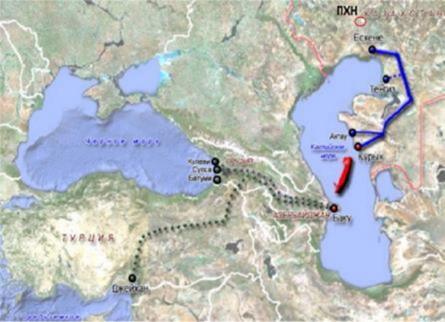
\includegraphics[width=0.6\textwidth]{assets/304}
	\caption*{Figure 1 - Location of the planned underground oil storage
facility located in Inder district of Atyrau region}
\end{figure}

\begin{multicols}{2}
{\bfseries Materials and methods.} The underground oil storage project will
help stabilize Kazakhstan\textquotesingle s oil production,
transportation and storage. The discovery of an old abandoned
underground salt mine, presents significant prospects and a number of
advantages of using the space of this mine for the construction of
underground oil storage. {[}3{]}

It is proposed to create with relatively low investment underground
storage in salt deposits, in the depleted salt mines of Inder. Inder is
located in Atyrau region, and on the way of main oil pipelines
Karachaganak-KTK, Atyrau-Samara. The technology of CCS has been tested
worldwide, i.e. storage in salt domes is cheaper, safer, less negative
impact on the environment, and there are practically no operating costs
compared to ground equipment.

The cost of storage is several times cheaper than above-ground storage
tanks. And due to the fact that oil will be stored at a depth of 300
meters (in the Caspian region 200 meters below sea level), it will
preserve the temperature regime and pressure for oil, and as a
consequence of preserving the quality of oil for a long time. {[}4{]}

Geographical location:

The mine\textquotesingle s location between major oil and gas fields and
its proximity to major transportation routes make it an ideal location
for a storage facility. This will reduce transportation costs and
provide easy access to the storage facility.

Safety and sustainability:

The underground location of the storage facility provides it with
protection from external influences such as weather or human factors,
which increases the safety and sustainability of the storage facility.

Unique geotechnical properties:

An underground salt mine has unique geotechnical characteristics that
can be ideally adapted to create an oil storage facility. For example,
salt is a stable and strong material, making it ideal for creating
secure walls and ceilings.

Cost-effectiveness:

Utilizing existing infrastructure reduces the cost of building a storage
facility and shortens the project timeline. This makes the project more
cost effective and competitive.

Reduced environmental impact: Underground storage minimizes negative
environmental impacts because it does not require a large land area and
does not create significant visual or environmental changes.

Based on the above factors, the use of an old salt mine for the
construction of an underground oil storage facility appears promising
and promises to bring significant benefits in terms of both economics
and the safety and sustainability of the oil infrastructure.

The estimated time and financial framework for converting the salt mine
to an oil storage facility is very important to understand the scope of
the project and its implementation. A timeframe of 3.5 years to convert
the mine and construct the infrastructure is realistic given the
complexity of the work and the amount of engineering involved.

Including the acquisition of geological information, study of the mine
condition, reanimation of its shafts, cleaning and repair works,
construction of infrastructure and facilities, laying of oil pipelines
and railroad tracks will ensure safe and efficient operation of the oil
storage facility.

The total cost of the project, estimated at \$370 million, also looks
realistic given the complexity and scale of the work. This is an
important investment decision that could bring significant benefits to
the oil and gas industry and the wider economy of the region. The
expected payback period of 6-7 years is reasonable and in line with
generally accepted investment standards.

{\bfseries Results and discussion.} Applying similar concepts and
experience to the project in Kazakhstan can ensure its successful
implementation. Applying successful practices and experience of other
countries to the project in Kazakhstan will reduce risks and increase
the chances of successful implementation of this innovative project.

This will help to balance the oil market, provide reserves in case of
crisis or temporary disruptions in production. Such storage facilities
can also reduce dependence on imports of oil products and ensure stable
functioning of the domestic market.

On the other hand, proponents of redirecting funds to the construction
of new export routes see this as a way to increase oil exports, which
could lead to higher oil revenues. However, it could also increase
dependence on foreign markets and increase risks in case of changes in
global oil demand or geopolitical tensions.

Large oil producers operating in Kazakhstan typically have their own
tank farms that are designed to meet the operational needs and manage
the flow of oil within their production operations. These tanks are
typically designed to store oil for short periods of time, such as a few
days, and do not provide long-term reserves or strategic stockpiles.

However, large oil storage facilities, as proposed by the President of
Kazakhstan, may have a more strategic function. They can be designed to
store significant volumes of oil for longer periods of time, allowing
the country to respond more flexibly to changes in supply and demand on
the world market, as well as to possible crisis situations, such as
temporary restrictions on oil exports or transportation.

The situation with the suspension of oil pumping through the
CPC\textquotesingle s main export route does highlight
Kazakhstan\textquotesingle s vulnerability to dependence on certain
transportation routes and markets. It also emphasizes the need to
develop alternative routes and infrastructure to diversify oil export
flows.

The repair pit contains slopes with specified slopes on both sides of
the main pipeline, while the pipeline is located in the ground with a
minimum wall thickness of at least 200-300 mm, and a flat bottom is
formed on both sides of the pipeline located in the ground to the width
of the excavator bucket. The technical result is that it is possible to
simplify the work by reducing manual labor as much as possible with
minimal environmental impact. The repair pit along the main pipeline 1
contains on both sides of the main pipeline 1 slopes 2 with specified
slopes (steepness). The main pipeline 1 is located in the ground 3 with
a minimum thickness of the soil wall of at least 200 -- 300 mm, and on
both sides of the main pipeline 1 located in the ground 3, a flat bottom
4 is formed for the width of the excavator bucket 5. The soil extracted
from the pit 6 is located at least 500 -- 700 mm from the edge of the
slopes 2 of the pit on both sides.

The method of developing a repair pit along the main pipeline 1, in
particular the oil pipeline, is that the repair pit is formed in the
form of a trench, and the fertile soil layer is previously removed,
which is formed in the form of a separate dump 7, the drainage strip is
cleared of shrubs and vegetation, the axis of the trench is broken down
and fixed on the terrain, which is made by end face when moving a
single-bucket excavator 5 along the axis of the newly laid oil pipeline
instead of the repaired one, while the soil 6 removed from the trench,
they are placed in the dump no closer than 0.5 -- 0.7 m from the edge of
the trench. When developing a trench with a single--bucket excavator 5,
hangers are placed along the axis of the trench (not shown in the
drawing) in front of it along the course of its movement and behind
along the already dug trench, and in rectilinear sections, along the
course of its movement, landmarks (hangers) with a height of 1 -- 3 m
are set every 30 - 50 m, to increase the accuracy of movement excavators
on curved sections relative to the trench within the curve along the
width of the tracks or along the width of the trench on both sides set
landmarks every 1-2 m. {[}5-6{]}

During the work carried out, it was found that the described method
ensures the precise movement of the excavator 5 along the underground
main pipeline 1 laid in the ground, and no strengthening of the slopes
is required, the ingress of soil from the dumps into the trench is
completely prevented and the fertile soil layer is preserved, which
fully allows restoring the environment after repair work on the main
pipeline and at the same time, minimize the use of manual labor to clean
the main pipeline under repair from the ground.

The construction of an oil storage facility can face various risks that
can affect the project. The main risks to be considered are:

Technical Risks:

Technical Problems: Unforeseen technical problems during construction or
operation can lead to delays and additional costs.

Process Disruption: Errors in design or construction could lead to
disruption of the oil storage process and jeopardize the safety of the
facility.

Environmental Risks:

Environmental Pollution: The need to comply with environmental standards
and prevent soil, water and air pollution during construction and
operation of an oil storage facility.

Oil Spill Risks: {[}7{]}

The possibility of oil spillage from tanks or pipelines can cause
serious environmental and health consequences.

Financial risks:

Oil price volatility: Changes in world oil prices may affect the oil
storage tank lease revenues and the overall profitability of the
project.

Credit Risk Risks: The need for project financing and possible delays or
non-repayment of loans may affect the financial position of the project.

Economic risks:

Oil market price risk: Since oil storage facility lease revenues may
depend on oil prices, changes in the oil market may significantly affect
the financial performance of the project.

The construction of large oil storage facilities may be one step towards
mitigating such crisis situations. Storing oil in strategic reserves
will help mitigate temporary disruptions in transportation and ensure
stability of supply in both domestic and foreign markets. It can also
help minimize revenue losses in case of suspension or restriction of
export supplies.

Consideration of alternative export routes is equally important.
Development of additional transportation corridors can reduce dependence
on one main route and reduce risks for the country\textquotesingle s
economy in case of such crises in the future.

Thus, a comprehensive analysis of the construction of oil storage
facilities and the development of alternative export routes will make it
possible to take into account all factors and peculiarities.

Construction of storage facilities for raw materials and fuel is a
necessary measure, because storage facilities provide coverage of
seasonal and daily fluctuations and consumption, technological needs and
export supplies. In order to mitigate crisis situations, oil-producing
countries primarily seek to build strategic reserves.

In the world the practice of construction of underground storage
facilities for hydrocarbon raw materials and fuels has been applied
since the Second World War. They store crude oil, gasoline, jet and
diesel fuel, natural gas, helium concentrate, marginal and unsaturated
hydrocarbons.

Underground oil storage facilities are the safest and most
environmentally friendly option for storing hydrocarbons. Since, very
often accidents occur during their operation of aboveground reservoirs.

Underground storages can be constructed in natural or artificial
cavities, depending on the purpose. Natural cavities are mainly used for
storing natural gas, while artificial cavities formed by
geotechnological methods, for example, in rock salt deposits, are used
for storing oil products.

Compared to above-ground tanks, underground storage facilities are
characterized by higher economic efficiency, reduced losses from
evaporation of light fractions of the product, low fire and explosion
hazards, absence of product leakage and low probability of groundwater
contamination, high resistance to earthquakes. Last but not least, they
have an undeniable environmental advantage.{[}8{]}

Reduced global demand for oil amid the coronavirus pandemic, as well as
Kazakhstan\textquotesingle s plans to redirect a significant share of
its oil exports to routes via the Caspian Sea, actualize the importance
of storage systems. The country needs storage facilities to respond
flexibly and efficiently to possible changes in domestic demand, to
price increases that may occur as a result of liberalization or the
creation of a single EAEU market. {[}9{]}.

{\bfseries Conclusions.} Providing safe and secure oil storage is an
important challenge for any country with oil resources or dependent on
oil imports.

The country\textquotesingle s needs for oil storage facilities are
determined by the following factors: economic growth, development of
transportation infrastructure, energy security, and seasonal
fluctuations in demand. The studied experience of countries in building
and using large oil storage facilities with developed oil and gas
industry - China, USA and South Korea is of practical value for the
development of strategy and plans in the field of oil and gas
infrastructure in Kazakhstan. The ability to adapt best practices and
technologies to local conditions and needs will create a more efficient
and sustainable infrastructure. Despite the obstacles and risks that may
arise during the construction and operation of an oil storage facility -
accidents, equipment downtime and leaks of oil products from the storage
facility, as well as market risks (changes in oil prices, demand for
storage services and other factors), it can be concluded that the
construction of an oil storage facility for Kazakhstan is a relevant and
important issue. Due to the fact that Kazakhstan is a major oil producer
and has significant export volumes, ensuring reliable and efficient
storage of oil products becomes a priority.

A comprehensive analysis and consideration of various factors, including
economic, technical, geopolitical and environmental aspects, will allow
us to decide whether to build oil storage facilities or direct resources
to the development of alternative export routes.
\end{multicols}

\begin{center}
{\bfseries Литература}
\end{center}


\begin{noparindent}
1.
Официальный сайт Президента Республики Казахстан.
URL:https://www.akorda.kz/ru/glava-gosudarstva-provel-vstrechu-s-obshchestvennostyu-atyrauskoy-oblasti-810283

2.
Дарибаева Н. Г. Анализ и оценка методов повышения эффективности систем
сбора, подготовки и транспортировки высоковязкой нефти // КазҰТУ
хабаршысы - Вестник КазНТУ -- 2015.- № 2. - С. 191-195.

3.
Шаяхметова К. О. Развитие нефтегазового комплекса как фактор повышения
конкурентоспособности Казахстана / Шаяхметова К. О., Данабаева А. И.
// Әл-Фараби атындағы КазҰУ Хабаршысы. - Вестник КазНУ им. Аль-Фараби.
- 2014. - № 1. - с. 58-61.

4.
Султанмуратов Н. Новый нефтяной кризис и перспективы Казахстана //
Казахстан в глобальных процессах. - 2015, - № 3. - С. 21-34.

5.
И. Галактионов. Резервы нефти в США. - Статья 20.05.2022 г. на сайте
https://bcs.ru/ .

6.
Шейнфельд С. Зарубежный опыт правового регулирования предоставления
земельных участков для целей недропользования: Зарубежный опыт //
Нефть, Газ и Право Казахстана, 2016 - № 4. -- С. 38-46.

7.
Ногайбаев М. А. Международный опыт формирования и управления
стратегическими запасами нефти в условиях рыночной экономики. // Л. Н.
Гумилев атындагы ЕУУ хабаршысынын экономика сериясы. - 2019. - № 1. -
С. 110-118. DOI:https://doi.org/10.32523/2079-620X-2019-1-110-120

8.Россия построит подземные нефтехранилища
https://undergroundexpert.info/opyt-podzemnogo-

stroitelstva/poslednie-sobytiya/rossiya-podzemnye-neftehranilishha/

9. Какое нефтехранилище нужно Казахстану.
https://petrocouncil.kz/kakoe-neftehranilishhe-nuzhno-kazahstanu/ .
\end{noparindent}

\begin{center}
{\bfseries References}
\end{center}

\begin{noparindent}
1. Oficial\textquotesingle nyj sajt Prezidenta Respubliki Kazahstan.
URL:
https://www.akorda.kz/ru/glava-gosudarstva-provel-vstrechu-s-obshchestvennostyu-atyrauskoy-oblasti-810283
{[}in Russian{]}

2. Daribaeva N. G. Analiz i otsenka metodov povysheniya effektivnosti
sistem sbora, podgotovki i

transportirovki vysokovyazkoi nefti. //
KazҰTU khabarshysy - Vestnik KazNTU -- 2015.- № 2. - S. 191-195. {[}in
Russian{]}

3. Shayakhmetova K. O. Razvitie neftegazovogo kompleksa kak faktor
povysheniya konkurentosposobnosti Kazakhstana / Shayakhmetova K. O.,
Danabaeva A. I. // Әl-Farabi atyndaғy KazҰU Khabarshysy. - Vestnik KazNU
im. Al\textquotesingle-Farabi. - 2014. - № 1. - S. 58-61. {[}in
Russian{]}

4. Sultanmuratov N. Novyi neftyanoi krizis i perspektivy Kazakhstana. //
Kazakhstan v global\textquotesingle nykh protsessakh. - 2015, - № 3. -
S. 21-34. {[}in Russian{]}

5. I. Galaktionov. Rezervy nefti v SShA. - Stat\textquotesingle ya
20.05.2022 g. na saite https://bcs.ru/ . {[}in Russian{]}

6. Sheinfel\textquotesingle d S. Zarubezhnyi opyt pravovogo
regulirovaniya predostavleniya zemel\textquotesingle nykh uchastkov dlya
tselei nedropol\textquotesingle zovaniya: Zarubezhnyi opyt //
Neft\textquotesingle, Gaz i Pravo Kazakhstana, 2016 - № 4. -- S. 38-46.
{[}in Russian{]}

7. Nogaibaev M. A. Mezhdunarodnyi opyt formirovaniya i upravleniya
strategicheskimi zapasami nefti v usloviyakh rynochnoi ekonomiki. // L.
N. Gumilev atyndagy EUU khabarshysynyn ekonomika seriyasy. - 2019. - №
1. - S. 110-118. DOI:https://doi.org/10.32523/2079-620X-2019-1-110-120
{[}in Russian{]}

8. Russia to build underground oil storage facilities.
https://undergroundexpert.info/opyt-podzemnogo-stroitelstva/poslednie-sobytiya/rossiya-podzemnye-neftehranilishha/
{[}in Russian{]}

9. What kind of oil storage facility Kazakhstan needs.
https://petrocouncil.kz/kakoe-neftehranilishhe-nuzhno-kazahstanu/ .
\end{noparindent}

\emph{{\bfseries Information about authors}}

\begin{noparindent}
Smailova N.T.-Doctor of Technical Sciences, Professor, , Kazakh
University of Technology and Business named after K. Kulazhanov, Astana,
Kazakhstan, e-mail: ganibek2006@mail.ru;

Popov A.Yu. - Doctor of Technical Sciences, Professor, Professor of the
Omsk State Technical University, Omsk, Russian Federation. e-mail:
popov\_a\_u@list.ru.
\end{noparindent}

\emph{{\bfseries Сведения об авторах}}

\begin{noparindent}
Смайлова Н.-Т.-доктор технических наук, профессор, Казахский университет
технологии и бизнеса им. К. Кулажанова, Астана, Казахстан, e-mail:
ganibek2006@mail.ru.

Попов А.Ю.-доктор технических наук, профессор, Омский государственный
технический университет, Омск, Российская федерация. e-mail:
popov\_a\_u@list.ru.
\end{noparindent}


